% Generated from paper002_manuscript_model_order_v1.1.md by scripts/build_paper002_submission_tex.py.
% The Markdown and BibTeX files remain the synchronized content sources.
\documentclass[10pt]{article}
\usepackage[a4paper,margin=25mm]{geometry}
\usepackage[T1]{fontenc}
\usepackage[utf8]{inputenc}
\usepackage{amsmath,amssymb}
\usepackage{graphicx}
\usepackage{booktabs,tabularx,array}
\usepackage{enumitem}
\usepackage{fancyvrb}
\usepackage{caption}
\usepackage[numbers,sort&compress]{natbib}
\usepackage{xurl}
\usepackage[colorlinks=true,allcolors=blue]{hyperref}
\setlength{\parindent}{0pt}
\setlength{\parskip}{0.55em}
\renewcommand{\arraystretch}{1.12}
\graphicspath{{figures/}}

\title{When Parameter Repair Is Not Enough: Failure-Conditioned Model-Order Expansion for Embodied Control}
\author{Seonhye Gu\thanks{This work was independently conducted by the author as personal research while affiliated with the AI-Based Surgical Robot Innovation Lab. The affiliation is provided for identification purposes only and does not imply official laboratory output, institutional endorsement, or sponsorship.}\\
\small AI-Based Surgical Robot Innovation Lab}
\date{}
\begin{document}
\maketitle


\begin{abstract}

An embodied controller can fail because the parameters of its predictive model are wrong or because the model omits a state variable required by the observed dynamics. The first case calls for parameter repair; the second calls for a change in model class. We study a restricted decision between these responses in an Isaac Sim surgical-reach environment. After a zero-order target model is exposed to persistent drift, its position-update coefficient is repaired on a shared Episode 1 trace. A preregistered adequacy gate then asks whether the remaining residual is persistent, directional, and better explained by a prepared constant-velocity alternative. Episode 2 compares frozen zero order, repaired zero order, gated constant velocity, and a velocity oracle while holding the Cartesian controller fixed. The confirmatory design used the first 10 statically eligible seeds from 40 fresh candidates, 10 fresh balanced drift conditions, and a fresh Isaac process for every seed-arm-condition cell. All 400 dynamic cells and 20 static-retention cells passed execution-validity checks. Relative to repaired zero order, gated constant velocity reduced mean true open-loop \(H=10\) prediction error by 10.806 mm (crossed-bootstrap 95\% CI [10.331, 11.360] mm improvement) and fixed-horizon final distance by 13.304 mm (95\% CI [12.982, 13.599] mm improvement). Both continuous outcomes favored the expanded model in 100/100 paired seed-condition cells. The secondary 20 mm resolution rate was 100\% versus 76\%. Static retention was 10/10 for both models. The gate fired on 100/100 persistent-drift cases and 0/100 static, observation-noise, and single-impulse controls. These results support a narrow claim: structured failure after within-class repair can justify activating a prepared higher-order target model and can improve prediction-linked control without nominal regression. They do not establish autonomous model invention, hardware transfer, or clinical validity.

\textbf{Keywords:} model adequacy, system identification, model order, structural adaptation, world models, embodied control, surgical simulation, preregistration

\end{abstract}

\section{Introduction}

Predictive models are useful only to the extent that their errors are compatible with the decisions made from them. In model-based control and reinforcement learning, an agent predicts future state, reward, or observation trajectories and uses those predictions to select actions. Contemporary world-model systems range from compact recurrent latent dynamics to large generative simulators \cite{ha2018world,hafner2019planet,hafner2025dreamerv3,hou2026survey}. Across this range, performance depends not only on fitting observed data but also on whether the fitted model remains reliable over the horizon used for action selection \cite{hafner2019planet,janner2019mbpo}.

When a prediction fails, parameter adaptation is a natural first response. A filter coefficient can be updated, a transition rate re-estimated, or network weights fine-tuned while preserving the represented state variables. This is parsimonious and often sufficient. It is not sufficient when the data-generating process depends on a dynamic variable absent from the model class. Classical system identification separates parameter estimation from model-structure and order selection \cite{ljung1999system,akaike1974identification}, and residual diagnostics ask whether unexplained temporal structure remains after fitting \cite{ljung1978lack}. Embodied learning systems face the same distinction, but the decision is consequential: an unnecessary expansion adds complexity and instability, whereas refusing a necessary expansion produces systematic forecast error.

Consider a target that is believed to be static. A zero-order model can update its current position estimate, but it cannot carry velocity as state. Under persistent drift, an aggressive update coefficient reduces one-step lag without producing the correct multi-step forecast. A first-order constant-velocity model can represent the missing mode. Activating it whenever an anomaly appears would be a weak solution, however, because observation noise and transient impulses also produce residuals. The relevant question is therefore not simply whether a larger model performs better. It is whether failure evidence that survives the best permitted within-class repair is sufficiently structured to warrant a specific prepared expansion.

We operationalize this question in an Isaac Sim surgical-reach task. The study uses a minimal target-dynamics model, not a learned visual representation: the model receives the three-dimensional target command and predicts its future position. This deliberate reduction isolates the adequacy decision from perception and policy learning. A shared Episode 1 trace exposes zero order to persistent drift and selects the best allowed position-update coefficient. A locked gate then tests persistence, directional consistency, and comparative fit of the constant-velocity class. Episode 2 evaluates four target-model arms on unseen directions, speeds, delays, and durations while the downstream controller is held fixed. Static retention and matched negative controls guard against expansion by default.

The confirmatory design was preregistered before fresh-data execution. It makes four contributions:

\begin{enumerate}[leftmargin=*]

\item It defines a failure-conditioned adequacy test that separates parameter repair from a prepared increase in target-dynamics model order.

\item It couples prediction to behavior by using each model's \(H=10\) forecast as the target of an otherwise identical controller.

\item It uses static-first seed selection, a complete crossed seed-condition grid, fresh-process execution, paired continuous endpoints, and explicit validity accounting.

\item It tests selectivity with nominal retention and matched persistent-drift, static, observation-noise, and impulse controls.

\end{enumerate}

The contribution is deliberately bounded. Velocity and constant-velocity extrapolation are supplied in advance. The experiment tests whether a prepared operator should be activated, not whether an agent can invent an arbitrary new state variable, causal ontology, or neural architecture.

\begin{figure}[htbp]
\centering
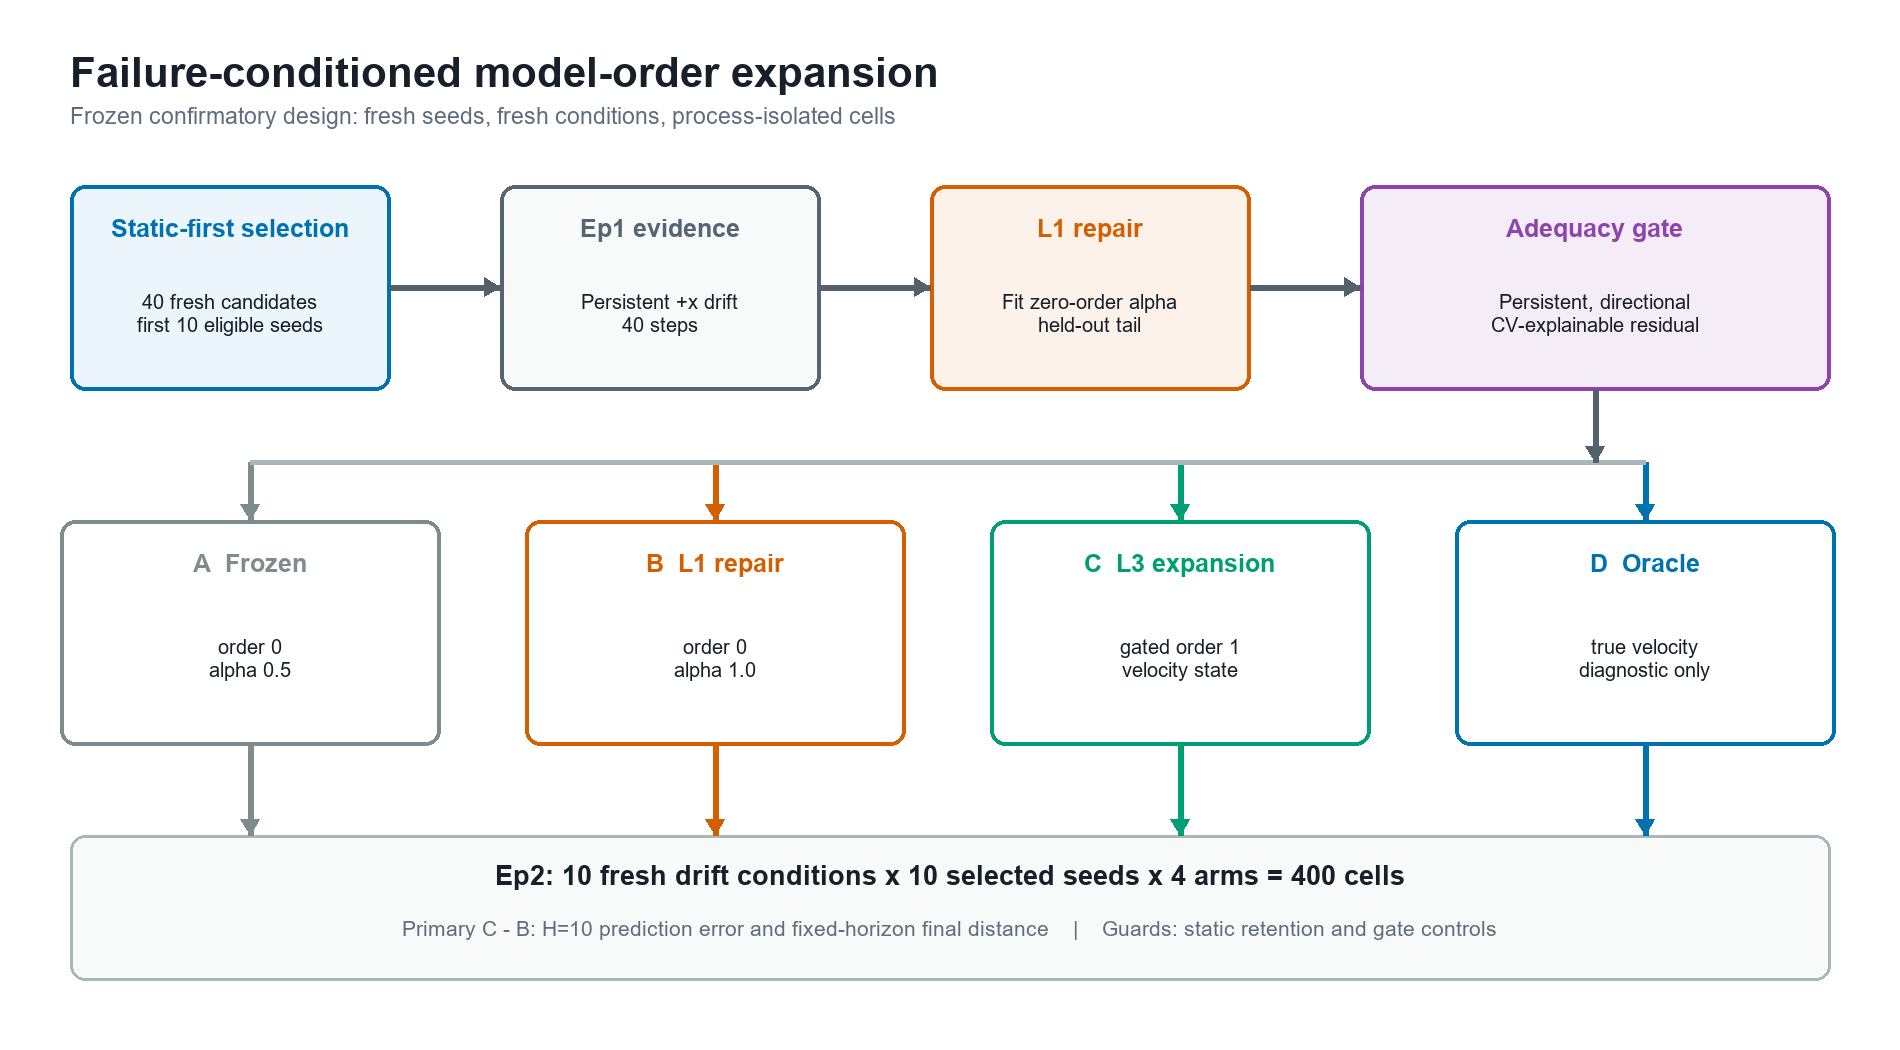
\includegraphics[width=0.96\linewidth]{figures/fig1_confirmatory_protocol.png}
\caption{Static-first confirmatory protocol. A common Episode 1 trace supports within-class repair and the locked adequacy test. The four target-model arms are then evaluated on the complete fresh seed-condition grid. C versus B is the primary contrast.}
\label{fig:1}
\end{figure}

\section{Related Work}

\subsection{Predictive World Models And Model-Based Control}

World models learn or encode how an environment evolves and make that information available to a policy or planner. Early neural formulations learned compressed spatial-temporal representations that could support policy learning inside imagined rollouts \cite{ha2018world}. PlaNet demonstrated online planning with learned latent dynamics from pixels \cite{hafner2019planet}, and DreamerV3 showed that a single world-model algorithm can support strong behavior across diverse domains \cite{hafner2025dreamerv3}. Robot-learning surveys now organize world models by roles including policy learning, planning, simulation, evaluation, and synthetic data generation \cite{hou2026survey}.

Most of this literature emphasizes how to learn an accurate model within a chosen architecture. Model-based policy optimization also emphasizes that model error compounds with rollout use and that an agent should limit reliance on a model when generalization is poor \cite{janner2019mbpo}. Our study asks a complementary, smaller question. Once failure persists after a permitted parameter repair, should the predictor retain its current order or activate a prepared higher-order state? The predictor here is intentionally interpretable, making the missing variable and its behavioral consequence directly auditable.

\subsection{Model Structure, Order, And Residual Adequacy}

System identification treats model structure, parameter estimation, and model validation as distinct choices \cite{ljung1999system}. Information criteria formalize a tradeoff between fit and complexity when selecting among candidate structures \cite{akaike1974identification}. Residual tests similarly treat remaining temporal dependence as evidence that a fitted model has not captured all predictable structure \cite{ljung1978lack}. These traditions motivate our repair-before-expansion order and the requirement that residual motion be predictable under the alternative class.

The present gate is not a general information criterion or a formal test of all possible misspecification. It compares two nested operational hypotheses in a controlled task: position-only dynamics and position-plus-velocity dynamics. The intervention is justified only when (i) the zero-order coefficient has been searched, (ii) motion is sustained and directional, and (iii) constant velocity improves short-window fit by a locked margin. Downstream prediction and control then test whether this structural diagnosis matters beyond the fitting trace.

\subsection{Modular And Continual Adaptation}

Mixture-of-experts models established that a gating mechanism can route inputs to specialized components \cite{jacobs1991experts}. Continual-learning systems extend this idea by composing modules and, in some cases, adding a module when local relevance or input-distribution evidence indicates that existing components are inadequate \cite{ostapenko2021lmc}. Recent embodied world-model work has moved modular adaptation to test time. TMoW updates routing and can integrate new world models for unseen or evolving domains \cite{jang2026tmow}. MuSix selects and updates world-model knowledge at multiple scales according to experiential distance \cite{jang2026musix}. Worldscape-MoE adds control-specific experts around shared dynamics to accommodate heterogeneous action modalities \cite{fang2026worldscape}.

These methods demonstrate that routing and expansion are useful mechanisms. They do not make expert addition itself novel here. Our empirical wedge is the decision before addition: failure must persist after a stronger parameter repair, match a specified alternative dynamic mode, improve prediction-linked behavior, preserve nominal control, and reject noise and impulse controls. The study thus tests when one prepared module is warranted rather than proposing a new general mixture architecture.

\subsection{Causal And Compositional Dynamics}

Structured world models can factor transition mechanisms so that sparse changes or interventions can be localized and adapted \cite{lei2023vcd}. This direction motivates a larger program in which residual patterns may suggest missing relations or variables. The present experiment is intentionally prior to that goal. It uses one known candidate variable and does not infer a causal graph. Its role is to establish an auditable adequacy-test cell in which the weaker model class is provably unable to express the relevant forecast and the prepared expansion has a direct behavioral consequence.

\section{Methods}

\subsection{Environment And Task}

Experiments use Isaac Sim 4.1 and the ORBIT-Surgical dual-arm reach environment \nolinkurl{Isaac-Reach-Dual-STAR-IK-Rel-Play-v0}. ORBIT-Surgical provides GPU-accelerated surgical robot-learning tasks for dVRK and STAR platforms \cite{yu2024orbit}. The present experiment uses only Cartesian target reaching; it does not evaluate tissue interaction, tool contact, or a clinical procedure.

The evaluated end effector follows a target command \(p_t\) in three-dimensional Cartesian space. The nominal mode M0 is static. In M1, a delay occurs after the locked onset and the target then drifts for a fixed number of steps:

\begin{align*}
\text{M0:}\quad p_{t+1} &= p_t, \\
\text{M1:}\quad p_{t+1} &= p_t + v,
\quad \text{during the condition-specific drift interval}.
\end{align*}

All arms use the same scripted Cartesian controller with gain 1.0, maximum action delta 0.08, and a 20 mm resolution tolerance. At each step, the target model's \(H=10\) forecast is installed as the policy command, the action is computed, and the true simulator command is restored before evaluation. Thus arm identity changes the forecast available to the controller but does not change controller parameters. The true future command, not the installed policy target, defines prediction error.

\subsection{Candidate Target Models}

The zero-order model maintains a filtered position estimate but has no velocity state. For position coefficient \(\alpha\),

\begin{align*}
\hat p_t &= \alpha p_t + (1-\alpha)\hat p_{t-1}, \\
\hat p_{t+H} &= \hat p_t.
\end{align*}

No value of \(\alpha\) can generate a nonzero open-loop target velocity. The prepared order-one model adds a filtered velocity estimate with coefficient \(\beta\):

\begin{align*}
\hat v_t &= \beta\left(p_t-p_{t-1}\right)
  +(1-\beta)\hat v_{t-1}, \\
\hat p_{t+H} &= \hat p_t + H\hat v_t,
  \quad \text{if the gate is active}.
\end{align*}

Before gate activation, the order-one arm returns the same position-only forecast as repaired zero order. The oracle uses the injected condition velocity and is diagnostic only.

\subsection{Episode 1 Evidence And Parameter Repair}

Episode 1 contains 40 steps of +x drift at 1.5 mm per step. The shared evidence is identical across arms. Zero-order repair searches \(\alpha \in \{0.25, 0.50, 0.75, 1.00\}\) and selects the value with the lowest held-out true \(H=10\) prediction error from step 20 onward. The expanded model's position and velocity coefficients are selected from the same Episode 1 evidence. No Episode 2 confirmatory outcome is used for model selection.

This ordering is important. Arm B is not a deliberately weak static baseline; it is the best model available within the locked zero-order family. Arm C must therefore improve over a completed within-class repair rather than over an unrepaired comparator.

\subsection{Structural Adequacy Gate}

The gate operates on an eight-step position window \(\mathcal{W}_t\). Let \(d_i=p_i-p_{i-1}\) denote target deltas, \(s_i=\lVert d_i\rVert_2\) their speeds, and \(m=\lvert\mathcal{W}_t\rvert\). It computes:

\begin{align*}
f_{\mathrm{active}}
  &= \frac{1}{m}\sum_{i\in\mathcal{W}_t}
     \mathbf{1}\!\left[s_i \ge 0.5\ \mathrm{mm/step}\right], \\
c_{\mathrm{dir}}
  &= \frac{\left\lVert\sum_{i\in\mathcal{W}_t}d_i\right\rVert_2}
          {\sum_{i\in\mathcal{W}_t}\lVert d_i\rVert_2}, \\
\operatorname{RMSE}_{0}
  &= \sqrt{\frac{1}{m}\sum_{i\in\mathcal{W}_t}\lVert d_i\rVert_2^2}, \\
\operatorname{RMSE}_{\mathrm{CV}}
  &= \sqrt{\frac{1}{m-1}\sum_{i\in\mathcal{W}_t\setminus\{i_0\}}
     \lVert d_i-d_{i-1}\rVert_2^2}, \\
I_{\mathrm{CV}}
  &= \frac{\operatorname{RMSE}_{0}-\operatorname{RMSE}_{\mathrm{CV}}}
          {\operatorname{RMSE}_{0}}.
\end{align*}

The gate fires only after at least four deltas are available and all locked conditions hold: mean speed at least 0.5 mm per step, active fraction at least 0.75, directional consistency at least 0.90, and constant-velocity improvement at least 0.50. This is a model-specific adequacy rule, not a generic anomaly score. The same rule is evaluated on persistent drift and on three matched controls: a static target, independent 0.2 mm observation noise, and a single impulse followed by rest.

\subsection{Experimental Arms}

\begin{table}[htbp]
\centering
\small
\begin{tabularx}{\textwidth}{@{}>{\raggedright\arraybackslash}X >{\raggedright\arraybackslash}X >{\raggedright\arraybackslash}X@{}}
\toprule
Arm & Target model & Role \\
\midrule
A & Frozen zero order, \(\alpha=0.5\) & Secondary unrepaired baseline \\
B & Repaired zero order, \(\alpha=1.0\) & Primary comparator \\
C & Gated constant velocity, \(\alpha=\beta=1.0\) & Primary intervention \\
D & Injected true velocity & Diagnostic oracle \\
\bottomrule
\end{tabularx}
\end{table}

A and B cannot represent velocity. C carries velocity only after the adequacy gate fires. D bounds model-side forecast error and indicates whether the shared controller can exploit velocity information; it is excluded from the primary contrast.

\subsection{Fresh Seeds And Drift Conditions}

Candidate seeds were fixed as integers 300 through 339. Static control was executed before any dynamic treatment. A seed was eligible only if its prefix reached the static target and its static-control trajectory remained within the 20 mm tolerance without reset or validity failure. The first 10 eligible seeds in numeric order were selected. This fixed-order quota prevents dynamic treatment performance from influencing inclusion.

Episode 2 contains 10 conditions C01-C10 with no exact pilot-condition reuse. The set balances positive and negative x and y directions and all four planar diagonals. Speeds range from 1.7 to 2.0 mm per step, delays from one to five steps, and durations from 20 to 23 steps. The primary grid is 10 selected seeds by 10 conditions by four arms, for 400 dynamic cells. Static retention adds one B and one C cell for each selected seed, for 20 cells. The exact condition table is reported in Supplementary Table S1.

\subsection{Process Isolation And Validity}

The experimental unit is one seed-arm-condition execution. An excluded engineering pilot batched multiple conditions inside a single Isaac process. Despite explicit reset seeds, preceding trajectories affected later reset states. The corrected pilot and confirmatory study therefore launch a fresh Isaac process for every cell. Within each seed-condition pair, all arms replay the same reset and prefix before branching.

The confirmatory run is invalid if the dynamic grid is incomplete, a selected prefix is not statically ready, paired branch-start end-effector states differ by more than 1 mm, branch commands differ by more than 1 micrometer, branch-start target distance exceeds 21 mm, an \(H=10\) prediction window is missing, drift exposure is incomplete, the environment resets unexpectedly, or the end effector enters the forbidden region. No failed or inconvenient cell may be silently removed. These rules were checked both per cell and in the aggregate result artifact.

\subsection{Outcomes And Estimands}

The primary population is the complete crossed set of selected seeds and fresh conditions. The primary analysis is intention-to-treat over every valid paired cell.

\begin{itemize}[leftmargin=*]

\item \textbf{H1 prediction:} mean C-minus-B true open-loop \(H=10\) target prediction error. The crossed-bootstrap 95\% interval upper endpoint must be at most -5 mm.

\item \textbf{H2 control:} mean C-minus-B end-effector distance at the fixed post-drift evaluation horizon. The 95\% interval upper endpoint must be at most -5 mm.

\item \textbf{H3 retention:} C static success must be at least 95\%, and the lower endpoint for C-minus-B static success must exceed -5 percentage points.

\item \textbf{H4 gate validity:} persistent-drift activation must be at least 90\%, and activation on each control must be at most 10\%.

\end{itemize}

The 20 mm resolution rate is secondary because the process-isolated pilot showed threshold saturation in the expanded arm. Diagnostic requirements additionally include at least 80\% success for C and D, reproduction of the Episode 1 parameter lock, and a valid execution grid. Confirmatory support requires all conjunctive criteria to pass.

\subsection{Statistical Analysis}

Seeds and conditions are crossed sampling factors rather than 100 independent replicates. For H1 and H2, the analysis independently resamples the 10 seed rows and 10 condition columns with replacement, evaluates the complete resampled cross product, and repeats this procedure 10,000 times using RNG seed 20260730. This procedure follows the logic of the pigeonhole bootstrap for crossed data \cite{owen2007pigeonhole}. We report the observed mean paired C-minus-B contrast, two-sided percentile 95\% interval, and fraction of paired cells favoring C. The secondary success contrast uses the same crossed resampling. Gate rates use Wilson score intervals \cite{wilson1927inference}. No multiplicity adjustment is applied because confirmatory support is conjunctive: every prespecified decision must pass.

\subsection{Preregistration, Software, And Compute}

The design, candidate seeds, condition set, selection rule, model candidates, gate thresholds, estimands, and decision criteria were frozen under immutable tag \nolinkurl{paper002-model-order-confirmatory-v1.0} before seeds 300-339 were executed. Pilot seeds and observations are excluded from every confirmatory estimate. There was no interim efficacy analysis or optional stopping.

Execution used container \nolinkurl{ghcr.io/higuseonhye/vessl-isaac-sim:4.1.0-v2} on one NVIDIA A100 SXM workspace with 11 vCPUs and 128 GB RAM. Isaac Sim ran headlessly with Fabric disabled to preserve the validated ORBIT-Surgical behavior. Derived statistics and figures are CPU reproducible from the committed JSON artifacts.

\section{Results}

\subsection{Accounting And Execution Validity}

Thirty-four of the 40 fixed candidates passed static eligibility. The first 10 eligible seeds were 300, 301, 302, 303, 304, 305, 307, 308, 310, and 311. All 400 dynamic cells and all 20 retention cells completed. The maximum paired branch-start end-effector and command gaps were both zero. Maximum branch-start target distance was 15.396 mm, below the 21 mm limit. Every prefix was ready, every prediction window was present, and every cell received full drift exposure. There were no unexpected environment resets or forbidden-region violations. The confirmatory run was valid.

\subsection{Episode 1 Reproduced Structural Inadequacy}

Zero-order repair selected \(\alpha=1.0\) but retained 15.000 mm held-out \(H=10\) prediction error. Constant velocity selected \(\alpha=\beta=1.0\) and reduced the same diagnostic error to numerical zero. The adequacy gate fired with active fraction 1.0, directional consistency 1.0, and constant-velocity fit improvement 1.0. The preregistered parameter and gate locks were reproduced on the fresh run.

\subsection{Prediction And Fixed-Horizon Control}

\begin{table}[htbp]
\centering
\small
\begin{tabularx}{\textwidth}{@{}>{\raggedright\arraybackslash}X >{\raggedright\arraybackslash}X >{\raggedright\arraybackslash}X >{\raggedright\arraybackslash}X >{\raggedright\arraybackslash}X@{}}
\toprule
Arm & n & \(H=10\) prediction error & Final distance & Resolution rate \\
\midrule
A frozen zero order & 100 & 20.081 mm & 20.388 mm & 39\% \\
B repaired zero order & 100 & 18.401 mm & 18.905 mm & 76\% \\
C gated constant velocity & 100 & 7.595 mm & 5.601 mm & 100\% \\
D oracle velocity & 100 & 0.000 mm & 4.087 mm & 100\% \\
\bottomrule
\end{tabularx}
\end{table}

For H1, C-minus-B prediction error was -10.806 mm (95\% CI [-11.360, -10.331] mm). For H2, C-minus-B final distance was -13.304 mm (95\% CI [-13.599, -12.982] mm). Both interval upper endpoints were below the locked -5 mm criterion. C had lower prediction error and lower final distance in all 100 paired seed-condition cells.

The secondary resolution-rate difference was +0.24 (95\% CI [+0.08, +0.45]): C resolved 100/100 cells and B resolved 76/100. A resolved 39/100. D resolved 100/100 and had zero forecast error. C's remaining 1.514 mm mean final-distance gap to D is consistent with the finite evidence window before gate activation.

\begin{figure}[htbp]
\centering
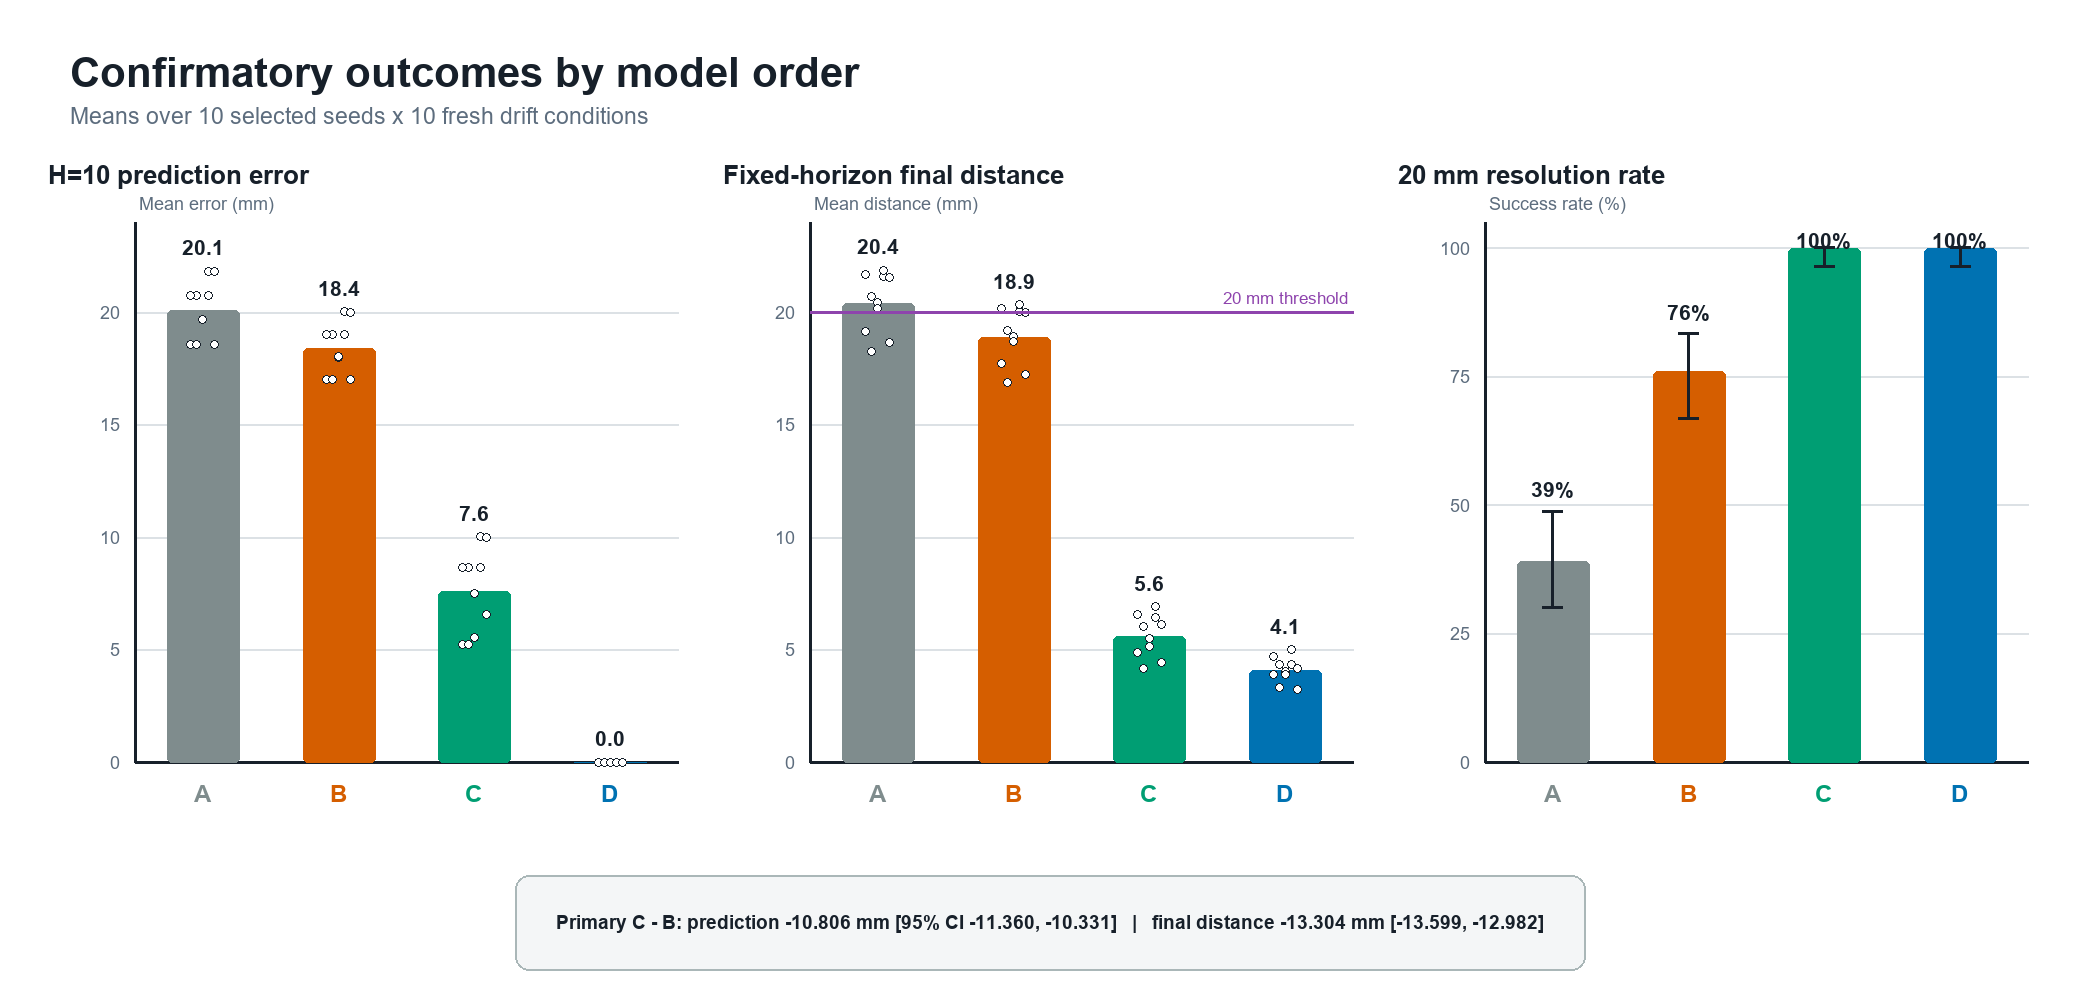
\includegraphics[width=0.96\linewidth]{figures/fig2_confirmatory_outcomes.png}
\caption{Arm-level confirmatory outcomes. Dots show condition means for the continuous endpoints; resolution bars include Wilson intervals. The 20 mm line is contextual and is not the H2 primary criterion.}
\label{fig:2}
\end{figure}

\subsection{Effects Across Fresh Conditions}

Condition-level C-minus-B prediction differences ranged from -12.462 to -9.998 mm. Final-distance differences ranged from -13.888 to -12.716 mm. C resolved all 10 seeds in every condition, while B resolved between 5 and 10 seeds depending on condition. No condition reversed either continuous primary effect.

\begin{figure}[htbp]
\centering
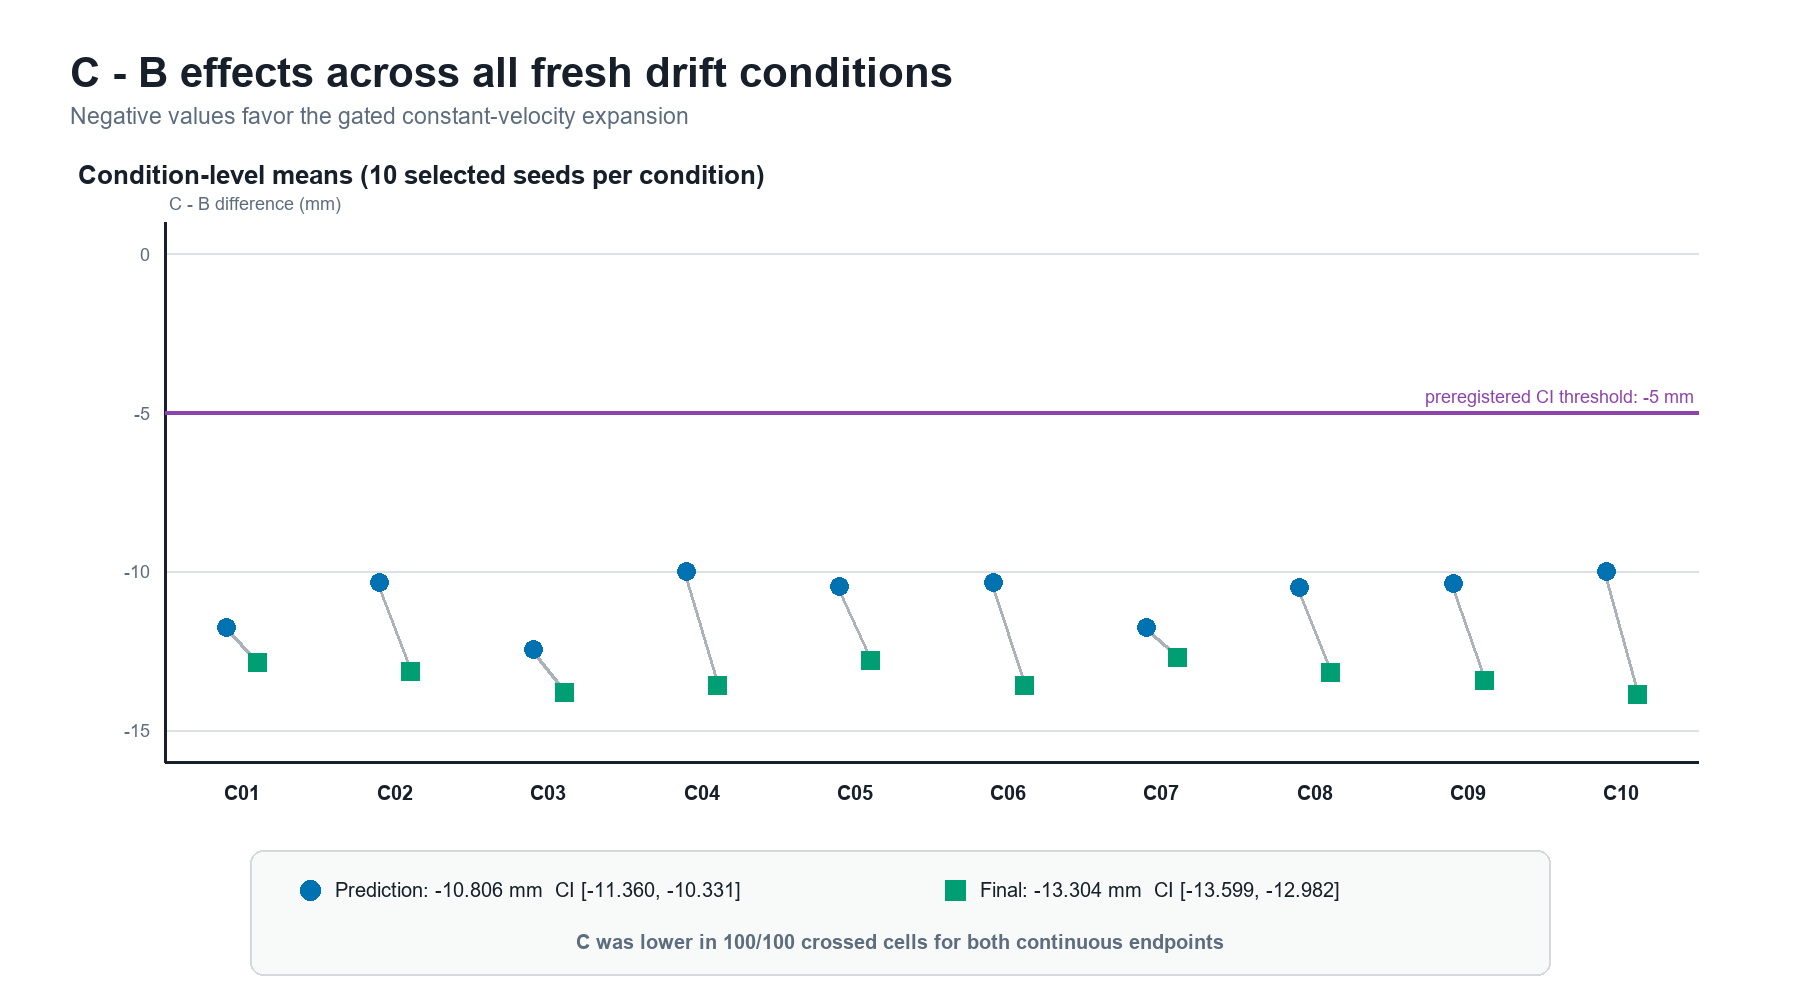
\includegraphics[width=0.96\linewidth]{figures/fig3_condition_effects.png}
\caption{Mean C-minus-B effects by fresh Episode 2 condition. Every condition lies beyond the -5 mm criterion for both endpoints. The formal decision uses the crossed-bootstrap interval over seeds and conditions.}
\label{fig:3}
\end{figure}

\subsection{Representative Mechanism Trace}

In the process-isolated seed 300/C04 branch, B and C begin from the same state and initially share the same position-only prediction. C's gate fires after enough directional evidence accumulates. Its \(H=10\) prediction error then falls from 20 mm to numerical zero, and end-effector distance decreases to 6.4 mm; B remains at 20 mm forecast error and finishes at 20.2 mm. The oracle receives velocity immediately and finishes at 4.5 mm. This trace is illustrative; every estimate above uses the complete crossed sample.

\begin{figure}[htbp]
\centering
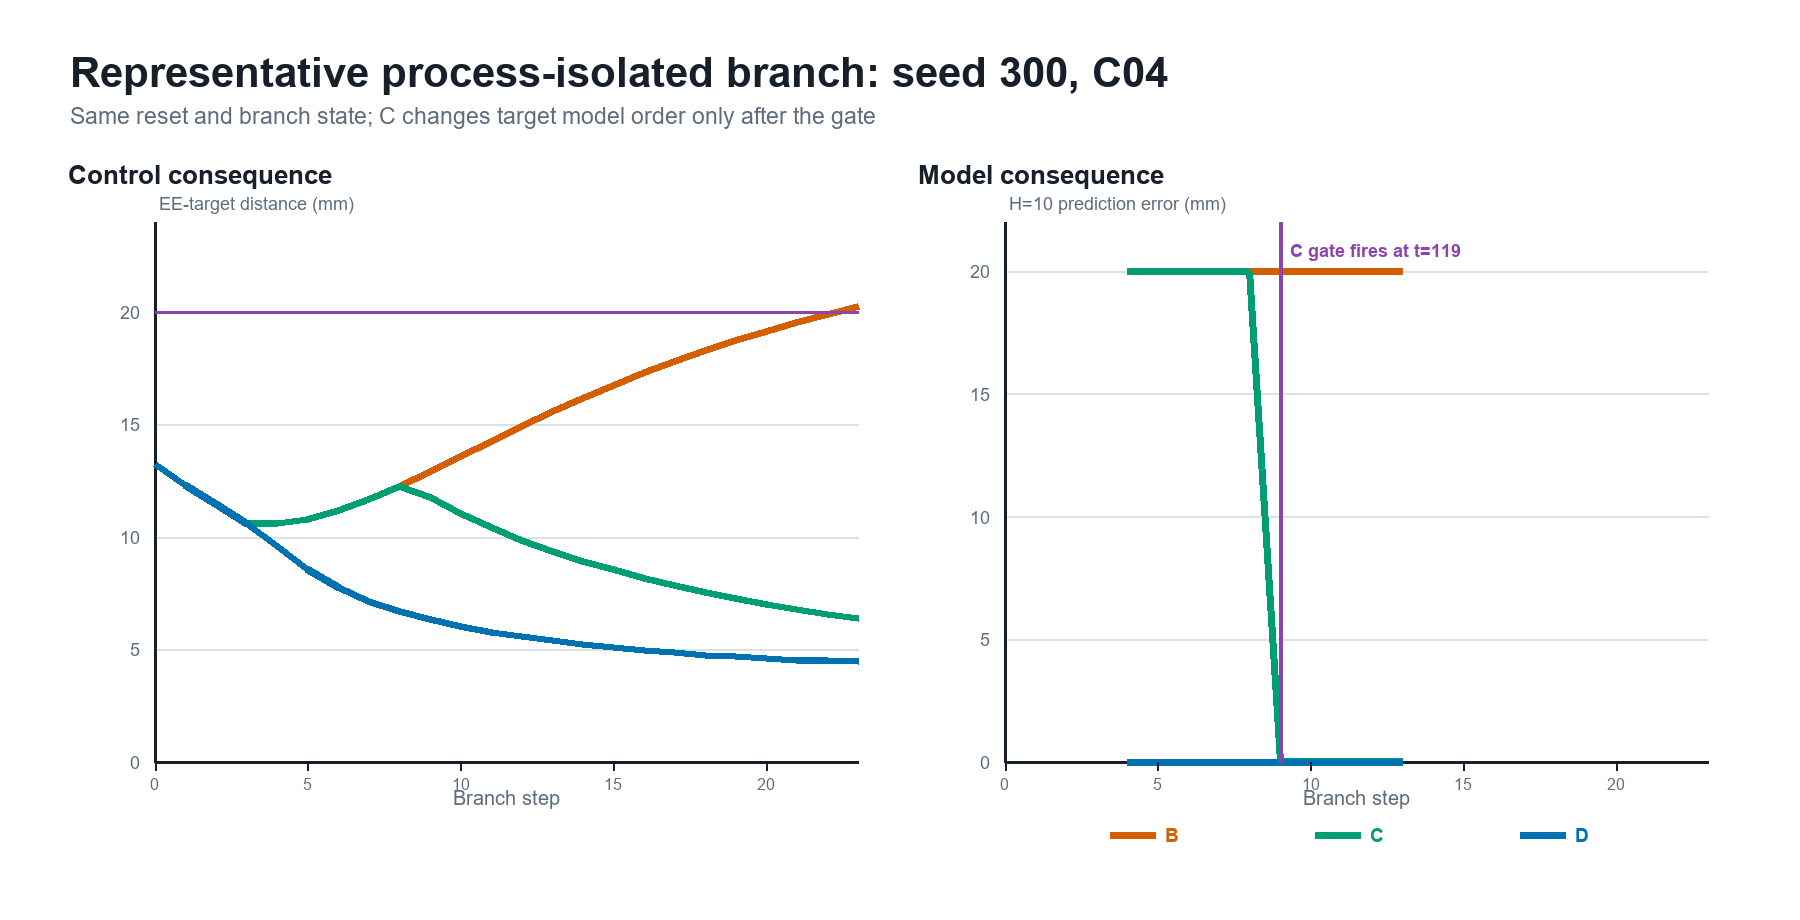
\includegraphics[width=0.96\linewidth]{figures/fig4_representative_trajectory.png}
\caption{Representative seed 300/C04 branch. The vertical line marks the first C gate activation. B, C, and D run in separate processes but replay exactly matched reset and branch states.}
\label{fig:4}
\end{figure}

\subsection{Static Retention And Gate Controls}

B and C each retained 10/10 static successes and had identical 1.501 mm mean final distance. The paired success-rate difference was 0.00 with 95\% interval [0.00, 0.00], passing the -5 percentage-point non-inferiority margin.

The gate fired in 100/100 persistent-drift evaluations (Wilson 95\% CI [96.30\%, 100\%]) and 0/100 evaluations for each of static target, observation noise, and single impulse (each Wilson upper 95\% bound 3.70\%). H3 retention and H4 gate validity passed.

\begin{figure}[htbp]
\centering
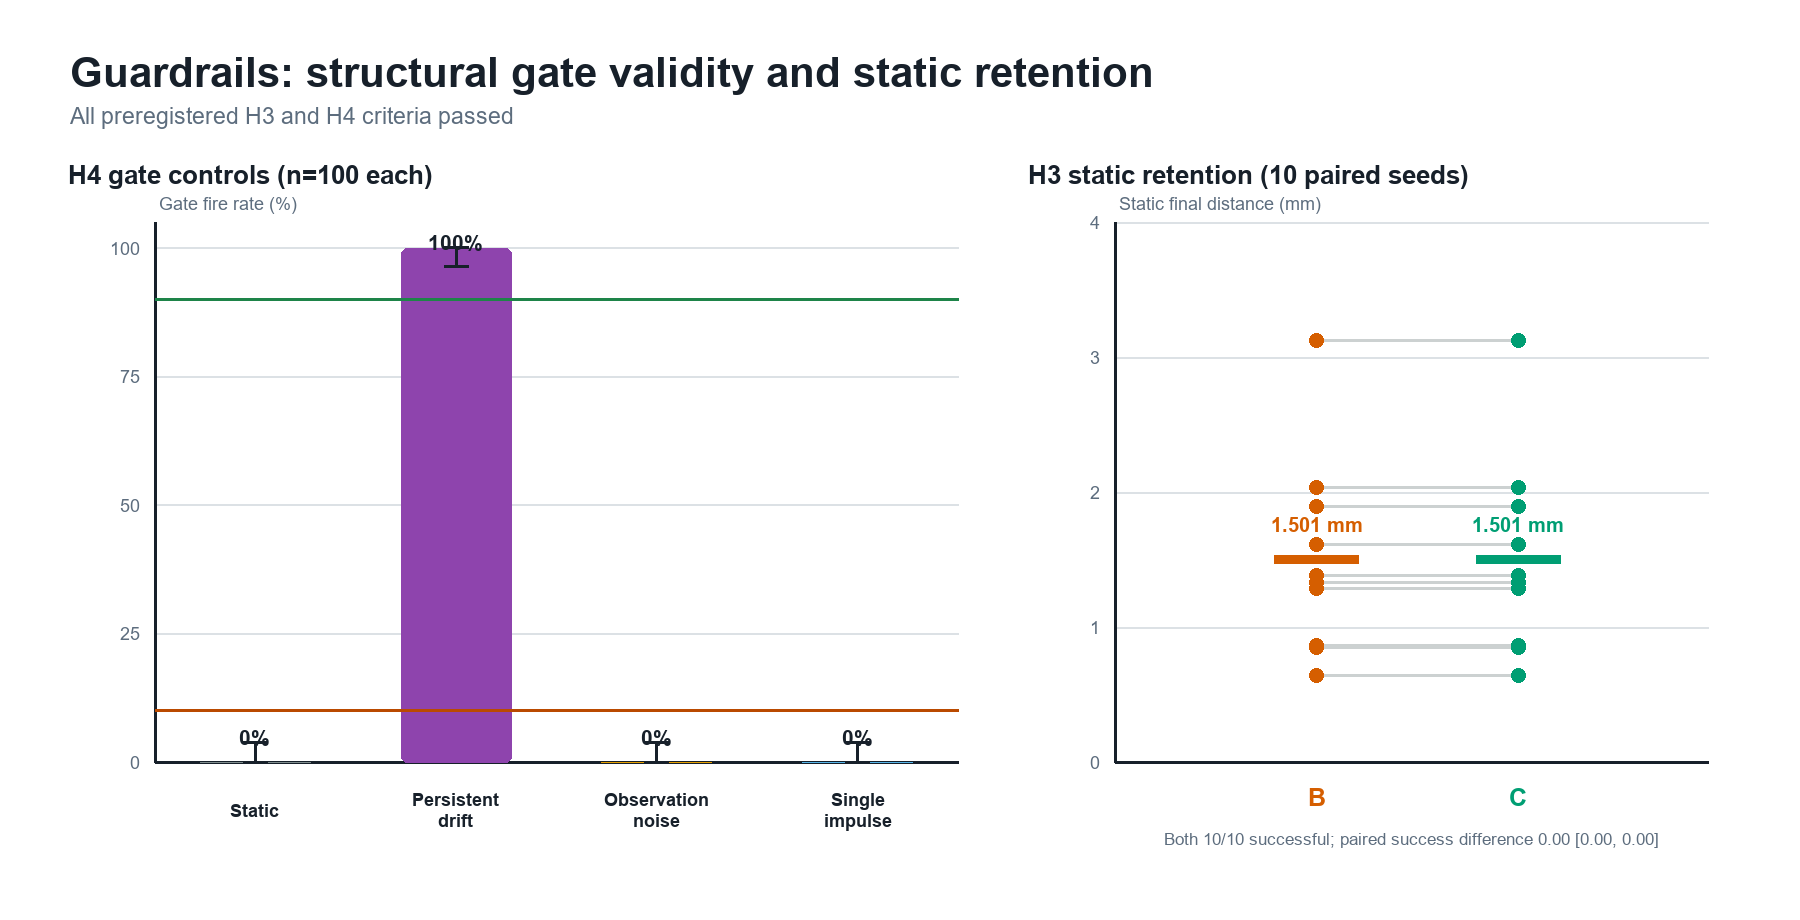
\includegraphics[width=0.96\linewidth]{figures/fig5_gate_and_retention.png}
\caption{The adequacy gate separates persistent directional drift from matched negative controls, while the expanded arm remains identical to repaired zero order on static retention.}
\label{fig:5}
\end{figure}

\subsection{Confirmatory Decision}

Every conjunctive field passed: execution validity, Episode 1 parameter lock, oracle behavior, C success floor, H1 prediction interval, H2 final-distance interval, H3 retention, H4 drift activation, and H4 control specificity. The preregistered confirmatory decision was positive.

\section{Discussion}

The experiment isolates a case in which a stronger parameter update is not a substitute for a missing state variable. Moving \(\alpha\) from 0.5 to 1.0 helps the zero-order model follow current position, improving prediction by 1.680 mm and final distance by 1.483 mm relative to frozen zero order. It cannot produce a nonzero H-step displacement. Adding a gated velocity state produces a much larger change: 10.806 mm lower forecast error and 13.304 mm lower final distance than the best allowed zero-order repair.

The prediction-to-control link is central. C is not rewarded only for fitting the Episode 1 trace. Its forecast becomes the target of an otherwise fixed controller, and the continuous control endpoint improves in every paired cell. The oracle shows that the controller can exploit correct velocity information; the remaining C-to-D gap is attributable primarily to evidence collection and gate latency. This design avoids claiming behavioral relevance from prediction error alone.

The controls delimit the trigger. A large residual is not sufficient evidence for a missing state because noise and impulses can also create error. Requiring sustained motion, directional agreement, and better alternative-class fit yielded complete activation on persistent drift and no activation on any matched control. Static retention further shows that the added state was not imposed on nominal trajectories. Together, these checks make the result an adequacy claim rather than a generic anomaly-response claim.

The study also clarifies how it relates to modern world-model research. It does not compete with high-capacity latent simulators on visual prediction or policy learning. Instead, it isolates a decision that such systems will eventually need to make: whether a poor forecast should be addressed by further optimization inside the current representation or by activating a representation with a different dynamic variable. Here that decision is transparent because the two candidate classes are simple and nested. Future learned systems may replace the hand-specified gate with probabilistic evidence while retaining the same experimental logic: repair first, demonstrate residual structure, test a prepared alternative out of sample, and verify behavioral benefit and nominal retention.

The positive result is conditional. For the tested persistent-drift family, failure that survives zero-order repair and is predictably explained by constant velocity warrants the prepared order-one model. It does not imply that every persistent failure is structural, that velocity is the right variable in other tasks, or that a system can discover the correct class without a candidate set.

\section{Limitations}

\begin{enumerate}[leftmargin=*]

\item \textbf{Prepared expansion.} Velocity and the constant-velocity operator are supplied in advance. The system selects between model classes; it does not invent a new variable or architecture.

\item \textbf{Minimal state observation.} The target command is observed directly. The experiment does not test perception, latent-state discovery, or uncertainty from images and force signals.

\item \textbf{Narrow dynamics family.} The hidden change is planar constant drift. Acceleration, multimodality, interaction, deformation, and contact dynamics are outside the confirmatory cell.

\item \textbf{Scripted controller.} Forecasts drive a deterministic Cartesian controller rather than a learned policy or general model-predictive controller. This improves causal isolation but limits behavioral scope.

\item \textbf{Selection-conditioned population.} The estimand applies to statically controllable resets under the frozen static-first rule, not to all simulator initializations.

\item \textbf{Single simulator and task.} Evidence comes from one ORBIT-Surgical reach task in Isaac Sim 4.1. The asset stack emitted known PhysX mass/inertia warnings, and no independent physical mass-property validation was performed.

\item \textbf{Rule-based gate.} Thresholds were locked after an excluded engineering pilot. Learned, probabilistic, and uncertainty-calibrated adequacy tests remain future work.

\item \textbf{No physical or clinical validation.} No tissue interaction, hardware robot, clinician, patient, or operating-room deployment was evaluated.

\end{enumerate}

The next scientific step is not to broaden the present claim by wording. It is to test the same repair-versus-expansion decision under new dynamic families, richer observations, learned controllers, and hardware measurement.

\section{Conclusion}

In a preregistered, process-isolated embodied-simulation experiment, a repaired zero-order target model remained structurally unable to forecast persistent drift. Activating a gated velocity-state expansion reduced \(H=10\) prediction error and fixed-horizon final distance by more than the locked 5 mm margins, with consistent benefit in every paired cell, no static regression, and no false activation on three negative controls. Failure after parameter repair can therefore support a restricted model-adequacy decision when the alternative class is prepared and the claim is guarded by prediction, control, retention, and specificity tests.

\section*{Declarations}

\textbf{Independent research and affiliation.} This work was independently conducted by Seonhye Gu as personal research while affiliated with the AI-Based Surgical Robot Innovation Lab. The affiliation is provided for identification purposes only and does not imply official laboratory output, institutional endorsement, or sponsorship.

\textbf{Funding and competing interests.} This study was conducted as independent personal research and does not claim institutional sponsorship. The author declares no competing interests related to this work.

\textbf{Author contributions.} Seonhye Gu was responsible for conceptualization, methodology, software, validation, formal analysis, investigation, data curation, visualization, manuscript preparation and revision, and project administration.

\textbf{AI-assisted tools.} AI-assisted tools supported software development and manuscript editing. The author reviewed the generated material, verified the reported analyses against the committed artifacts, and accepts full responsibility for the work.

\section*{Ethics, Data, Code, And Reproducibility}

No human participants, animals, patient data, or clinical workflows were used. The experiment is entirely simulated. Surgical terminology identifies the robot platform and benchmark family and must not be interpreted as clinical validation.

The preregistration, frozen configuration, complete records and trajectories, analysis code, figure manifest, and checksums are archived in the \href{\detokenize{https://github.com/higuseonhye/research-os}}{public research repository}. Pilot results remain archived but are excluded from confirmatory estimates.

\bibliographystyle{unsrtnat}

\bibliography{paper002_references_v1.1}

\end{document}
